% Created 2014-06-02 Mon 15:17
\documentclass[bigger, presentation]{beamer}
\usepackage[utf8]{inputenc}
\usepackage[T1]{fontenc}
\usepackage{fixltx2e}
\usepackage{graphicx}
\usepackage{longtable}
\usepackage{float}
\usepackage{wrapfig}
\usepackage{soul}
\usepackage{textcomp}
\usepackage{marvosym}
\usepackage{wasysym}
\usepackage{latexsym}
\usepackage{amssymb}
\usepackage{hyperref}
\tolerance=1000
\usepackage{minted}
\usetheme{Frankfurt}   
\usecolortheme[RGB={0,104,139}]{structure}%deepskyblue
\usefonttheme{serif}  % or try serif, structurebold, ...
\setbeamertemplate{navigation symbols}[horizontal]
\setbeamertemplate{caption}[numbered]
\useinnertheme{rounded}
\setbeamercovered{transparent}
\usepackage{pgfpages}
\pgfpagesuselayout{resize to}[physical paper width=8in, physical paper height=6in]
\logo{
\includegraphics[height=1cm,width=1cm]{iitb-logo.jpeg}}
\usepackage{array}
\usepackage{graphicx}
\usepackage{hyperref}
\usepackage[english]{babel}
\usepackage{pxfonts}
\usepackage{listings}
\lstset{numbers=left,numbersep=6pt,numberstyle=\tiny,showstringspaces=false,aboveskip=-50pt,frame=leftline,keywordstyle=\color{black},commentstyle=\color{orange},stringstyle=\color{black},}
\date{today}
\subtitle{because we like silly names | session 2(intermediate)}
\institute{Indian Institute of Technology Bombay}
\providecommand{\alert}[1]{\textbf{#1}}

\title{git}
\author{Sachin}
\date{\today}
\hypersetup{
  pdfkeywords={git, version control},
  pdfsubject={my first presentation made in org mode},
  pdfcreator={Emacs Org-mode version 7.9.3f}}

\begin{document}

\maketitle

\section{Session1}
\label{sec-1}
\begin{frame}
\frametitle{Last session}
\label{sec-1-1}


\begin{itemize}
\item Introduction
\item Initialize a \texttt{git} repo
\item Add a file/all files
\item Commit a file
\item Status of a project
\item Update a file
\item Log of commits
\item GIT Branch
\end{itemize}
\end{frame}
\begin{frame}
\frametitle{Last session}
\label{sec-1-2}
\begin{block}{Commands:Local}
\label{sec-1-2-1}

\begin{itemize}
\item git init
\item git add <FILENAME>
\item git commit -m ``MESSAGE''
\item git diff <FILENAME>
\item git add -u
\item git status
\item git log
\item git log --oneline
\item git log --graph --decorate --oneline
\end{itemize}
\end{block}
\end{frame}
\begin{frame}
\frametitle{Last session}
\label{sec-1-3}
\begin{block}{Commands:GitHub}
\label{sec-1-3-1}

\begin{itemize}
\item git add remote origin <REMOTE URL>
\item git remote -v
\item git push -u origin master
\item git push
\end{itemize}
        
\end{block}
\end{frame}
\section{clone/pull/fetch}
\label{sec-2}
\begin{frame}[fragile]
\frametitle{\texttt{clone, pull}}
\label{sec-2-1}

   
   \emph{If you have to download the repo from GitHub}

\begin{minted}[]{sh}
git clone <REMOTE_URL>
\end{minted}


\begin{minted}[]{sh}
git clone https://github.com/psachin/octo.git
\end{minted}


   \emph{If you want to sync local repo with GitHub}

\begin{minted}[]{sh}
git pull
\end{minted}
\end{frame}
\section{Branch}
\label{sec-3}
\begin{frame}
\frametitle{GIT branch: What is that?}
\label{sec-3-1}



  \begin{figure}[htb]
  \centering
  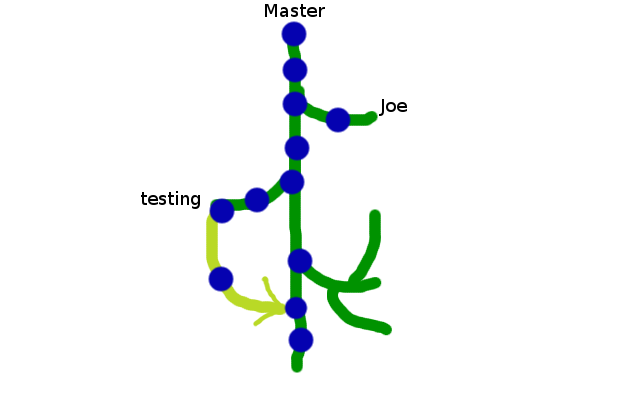
\includegraphics[width=10cm,angle=0]{./branch.png}
  \caption{\label{fig:branch}Git branches}
  \end{figure}
\end{frame}
\begin{frame}[fragile]
\frametitle{Know your current working branch}
\label{sec-3-2}



\begin{minted}[]{sh}
git branch
\end{minted}
\end{frame}
\begin{frame}[fragile]
\frametitle{Create a new branch}
\label{sec-3-3}



\begin{minted}[]{sh}
git branch devel
\end{minted}
\end{frame}
\begin{frame}[fragile]
\frametitle{Switch branch}
\label{sec-3-4}



\begin{minted}[]{sh}
git checkout <BRANCH_NAME>
\end{minted}


\begin{minted}[]{sh}
git checkout devel
\end{minted}
\end{frame}
\begin{frame}[fragile]
\frametitle{Merge branch}
\label{sec-3-5}


   \emph{Switch to target branch}

\begin{minted}[]{sh}
git checkout master
\end{minted}

   \emph{Merge}

\begin{minted}[]{sh}
git merge devel
\end{minted}
\end{frame}
\begin{frame}[fragile]
\frametitle{Push branch}
\label{sec-3-6}



\begin{minted}[]{sh}
git push origin devel
\end{minted}
\end{frame}
\section{GitHub}
\label{sec-4}
\begin{frame}
\frametitle{Hosting your code}
\label{sec-4-1}



  \begin{figure}[htb]
  \centering
  
\includegraphics[width=10cm,angle=0]{./github.png}
  \caption{\label{fig:GitHub}GitHub}
  \end{figure}
\end{frame}
\begin{frame}
\frametitle{Collaborate using GitHub}
\label{sec-4-2}


\begin{itemize}
\item fork
\item clone
\item commit \& push
\item pull request
\end{itemize}
\end{frame}
\section{3 R's}
\label{sec-5}
\begin{frame}
\frametitle{Reset/Reflog/Revert}
\label{sec-5-1}

 
\begin{itemize}
\item Reset
\item Reflog
\item Revert
\end{itemize}
\end{frame}
\begin{frame}[fragile]
\frametitle{Get back to old commit hash}
\label{sec-5-2}
\begin{block}{With no history}
\label{sec-5-2-1}


\begin{minted}[]{sh}
git reset --hard <COMMIT HASH>
\end{minted}
\end{block}
\begin{block}{With history}
\label{sec-5-2-2}


\begin{minted}[]{sh}
git revert <COMMIT HASH>
\end{minted}
\end{block}
\end{frame}
\section{Host}
\label{sec-6}
\begin{frame}
\begin{block}{Hosting sites}
\label{sec-6-1-1}

\begin{itemize}
\item github.com
\item gitlab.com
\item bitbucket.org
\item sourceforge.net
\end{itemize}
     
\end{block}
\end{frame}
\section{Question}
\label{sec-7}
\begin{frame}[fragile]

   
\includegraphics[width=5cm,angle=0]{./questions.png}
   

\begin{minted}[]{sh}
isachin@iitb.ac.in
\end{minted}
\end{frame}
\section{Refs/links}
\label{sec-8}
\begin{frame}
\begin{block}{Reference}
\label{sec-8-1-1}

\begin{itemize}
\item \emph{Pro Git}
\end{itemize}
\end{block}
\begin{block}{Links}
\label{sec-8-1-2}

\begin{itemize}
\item \href{http://www.emacswiki.org/emacs/}{http://git-scm.com/}
\end{itemize}
\end{block}
\end{frame}

\end{document}
